\level{1}{Descrizione delle classi}
	\level{2}{Legenda}
		Viene riportata in seguito la legenda riguardante i diagrammi presenti in tale sezione. Sono stati utilizzati colori diversi per classi con compiti diversi:
		\begin{itemize}
			\item le classi in grigio rappresentano librerie o moduli esterni, sui quali non abbiamo alcuna responsabilità;
			\item le classi in arancione sono tutte le classi factory presenti e le interfacce che esse implementano;
			\item le classi in verde sono le classi del modello che implementano l'interfaccia Updater e l'interfaccia Updater stessa;
			\item le classi in rosa sono le classi del modello che implementano la classe ChartImpl.
		\end{itemize}
	\level{2}{Norris}
		In questa sezione sono presenti le descrizioni di tutte le classi presenti all'interno del prodotto Norris. Queste sono state suddivise in base al componente nelle quali sono contenute.
		
		\level{3}{Design pattern utilizzati}
			Nella progettazione delle classi di Norris abbiamo deciso di utilizzare alcuni design pattern. Riportiamo di seguito una loro breve descrizione e il contesto nel quale sono stati utilizzati.
			\level{4}{Observer}
				L'Observer è un pattern comportamentale che ha lo scopo di monitorare lo stato di diversi oggetti legati ad un soggetto.
				Per la descrizione del pattern e dei vantaggi derivanti dalla sua applicazione si rimanda all'appendice \nameref{app:observer}.
				\level{5}{Contesto di utilizzo}
					Il pattern Observer si basa sugli oggetti “osservabili” e sugli “osservatori”.\\
					Le interfacce che che estendono Observable sono le seguenti:
					\begin{itemize}
						\item DataModel::ChartModel;
						\item DataModel::NorrisModel.
					\end{itemize}
					L'interfaccia Observer è implementata dalla classe EventEmitter fornita da Node.js.
			\level{4}{Bridge}
				Il Bridge è un pattern strutturale pensato per separare l'interfaccia di una classe dalla sua implementazione.\\
				Per la descrizione del pattern e dei vantaggi derivanti dalla sua applicazione si rimanda all'appendice \nameref{app:bridge}.
				\level{5}{Contesto di utilizzo}
					In Norris questo pattern viene utilizzato nel package InternalAPIManager per separare l'implementazione dei chart (presente nel package DataModel) dall'interfaccia fornita allo sviluppatore.
			\level{4}{Dependency Injection}
				Dependency Injection è un pattern architetturale il cui scopo è separare il comportamento di una componente dalla risoluzione delle sue dipendenze.\\
				Per la descrizione del pattern e dei vantaggi derivanti dalla sua applicazione si rimanda all'appendice \nameref{app:dependencyinjection}.
				\level{5}{Contesto di utilizzo}
					Il pattern Dependency Injection viene utilizzato con le classi che implementano le seguenti interfacce:
					\begin{itemize}
						\item ExternalAPIManager::EndpointFactory, inietta in ExternalAPIManager::ExternalAPIController le dipendenze verso i diversi Endpoint;
						\item DataModel::ChartFactory, inietta in DataModel::ChartImpl le  corrispondenze tra i tipi di grafico e le rispettive classi factory;
						\item DataModel::Updater, inietta in DataModel::ChartImpl le corrispondenze tra i diversi tipi di aggiornamenti e le classi che li implementano.
					\end{itemize}
			\level{4}{Singleton}
				Il Singleton è un pattern creazionale il cui scopo è permettere la creazione di una sola istanza di una classe, nonchè di fornire un punto di accesso globale ad essa.\\
				Per la descrizione del pattern e dei vantaggi derivanti dalla sua applicazione si rimanda all'appendice \nameref{app:singleton}.
				\level{5}{Contesto di utilizzo}
					Le classi che implementano il Singleton sono quelle che si occupano di creare i diversi tipi di grafici. Le riportiamo di seguito:
					\begin{itemize}
						\item DataModel::BarChartFactory;
						\item DataModel::LineChartFactory;
						\item DataModel::MapChartFactory;
						\item DataModel::TableFactory;
						\item ExternalAPIManager::ChartEndpoitFactory;
						\item ExternalAPIManager::AuthenticationEndpointFactory;
						\item ExternalAPIManager::ListEndpointFactory.
					\end{itemize}
			\level{4}{Abstract Factory}
				Il pattern creazionale Abstract Factory si occupa di fornire un'interfaccia per la creazione di famiglie di prodotti, senza dover specificare classi concrete.\\
				Per la descrizione del pattern e dei vantaggi derivanti dalla sua applicazione si rimanda all'appendice \nameref{app:abstractfactory}.
				\level{5}{Contesto di utilizzo}
					Gli elementi che implementano Abstract Factory sono quelli indicati in seguito.
					\begin{itemize}
					\item Interfacce:
						\begin{itemize}
							\item ChartFactory, con cui vengono generati i diversi tipi di grafici;
							\item ExternalAPIManager::EndpointFactory, con cui sono generati i diversi tipi di controller dei grafici.
						\end{itemize}
					\item Classi:
						\begin{itemize}
							\item DataModel::BarChartFactory;
							\item DataModel::LineChartFactory;
							\item DataModel::MapChartFactory;
							\item DataModel::TableFactory;
							\item ExternalAPIManager::ChartEndpointFactory;
							\item ExternalAPIManager::AuthenticationEndpointFactory;
							\item ExternalAPIManager::ListEndpointFactory.
						\end{itemize}
					\end{itemize}
					
		\level{1}{Norris}
    \level{2}{Specifica dei componenti}
	Nella presente sezione è stata riportata e documentata la progettazione di dettaglio del \insglo{prodotto} \insglo{Norris}. Si noti che tale progettazione deriva direttamente dalla progettazione architetturale che può essere trovata all'interno del documento \insdoc{Specifica Tecnica v4.00}. I risultati ottenuti sono stati organizzati e presentati secondo la seguente struttura:
	\begin{enumerate}
		\item vengono innanzitutto presentate le varie classi che sono state individuate. Per ognuna di esse si indica il nome, il tipo, l'eventuale astrattezza, la visibilità e il fatto che estenda altre classi oppure no. In aggiunta a ciò, viene presentata una descrizione completa del ruolo e delle responsabilità della classe oltre a una documentazione completa riguardante tutti gli attributi e i metodi presenti all'interno.
		\item in secondo luogo vengono presentati i diagrammi di sequenza, che hanno lo scopo di descrivere scenari (determinate sequenze di azioni in cui tutte le scelte sono già state effettuate). Essi vengono usati per descrivere le relazioni che intercorrono, in termini di messaggi, tra attori, oggetti ed entità del sistema \insglo{Norris}.
	\end{enumerate}
	Le regole che sono state rispettate, gli strumenti che sono stati usati e le procedure che sono state effettuate possono essere trovate all'interno del documento \insdoc{Norme di Progetto v6.00}.
    \level{3}{Classi}
    	In tale sezione sono riportate delle descrizioni dettagliate delle classi individuate all'interno del documento \insdoc{Specifica Tecnica v4.00}. Tali classi sono presentate e organizzate in modo gerarchico, mantenendo una suddivisione per \insglo{package} di appartenenza.
        \level{1}{Norris}
    \level{2}{Specifica dei componenti}
	Nella presente sezione è stata riportata e documentata la progettazione di dettaglio del \insglo{prodotto} \insglo{Norris}. Si noti che tale progettazione deriva direttamente dalla progettazione architetturale che può essere trovata all'interno del documento \insdoc{Specifica Tecnica v4.00}. I risultati ottenuti sono stati organizzati e presentati secondo la seguente struttura:
	\begin{enumerate}
		\item vengono innanzitutto presentate le varie classi che sono state individuate. Per ognuna di esse si indica il nome, il tipo, l'eventuale astrattezza, la visibilità e il fatto che estenda altre classi oppure no. In aggiunta a ciò, viene presentata una descrizione completa del ruolo e delle responsabilità della classe oltre a una documentazione completa riguardante tutti gli attributi e i metodi presenti all'interno.
		\item in secondo luogo vengono presentati i diagrammi di sequenza, che hanno lo scopo di descrivere scenari (determinate sequenze di azioni in cui tutte le scelte sono già state effettuate). Essi vengono usati per descrivere le relazioni che intercorrono, in termini di messaggi, tra attori, oggetti ed entità del sistema \insglo{Norris}.
	\end{enumerate}
	Le regole che sono state rispettate, gli strumenti che sono stati usati e le procedure che sono state effettuate possono essere trovate all'interno del documento \insdoc{Norme di Progetto v6.00}.
    \level{3}{Classi}
    	In tale sezione sono riportate delle descrizioni dettagliate delle classi individuate all'interno del documento \insdoc{Specifica Tecnica v4.00}. Tali classi sono presentate e organizzate in modo gerarchico, mantenendo una suddivisione per \insglo{package} di appartenenza.
        \level{1}{Norris}
    \level{2}{Specifica dei componenti}
	Nella presente sezione è stata riportata e documentata la progettazione di dettaglio del \insglo{prodotto} \insglo{Norris}. Si noti che tale progettazione deriva direttamente dalla progettazione architetturale che può essere trovata all'interno del documento \insdoc{Specifica Tecnica v4.00}. I risultati ottenuti sono stati organizzati e presentati secondo la seguente struttura:
	\begin{enumerate}
		\item vengono innanzitutto presentate le varie classi che sono state individuate. Per ognuna di esse si indica il nome, il tipo, l'eventuale astrattezza, la visibilità e il fatto che estenda altre classi oppure no. In aggiunta a ciò, viene presentata una descrizione completa del ruolo e delle responsabilità della classe oltre a una documentazione completa riguardante tutti gli attributi e i metodi presenti all'interno.
		\item in secondo luogo vengono presentati i diagrammi di sequenza, che hanno lo scopo di descrivere scenari (determinate sequenze di azioni in cui tutte le scelte sono già state effettuate). Essi vengono usati per descrivere le relazioni che intercorrono, in termini di messaggi, tra attori, oggetti ed entità del sistema \insglo{Norris}.
	\end{enumerate}
	Le regole che sono state rispettate, gli strumenti che sono stati usati e le procedure che sono state effettuate possono essere trovate all'interno del documento \insdoc{Norme di Progetto v6.00}.
    \level{3}{Classi}
    	In tale sezione sono riportate delle descrizioni dettagliate delle classi individuate all'interno del documento \insdoc{Specifica Tecnica v4.00}. Tali classi sono presentate e organizzate in modo gerarchico, mantenendo una suddivisione per \insglo{package} di appartenenza.
        \input{Classi/Norris.tex}

    \level{3}{Classi aggiuntive}
        Per quanto riguarda le classi aggiuntive riguardanti che implementano i tipi “ChartSettings” e “ChartUpdate” si faccia riferimento all'appendice \nameref{app:schemi}, nella quale sono presenti gli schemi \insglo{JSON} di tali oggetti.
        \input{Classi/NorrisAggiuntive.tex}

    \level{2}{Diagrammi di sequenza}
    	In tale sezione vengono presentati i diagrammi di sequenza, che hanno lo scopo di descrivere scenari (determinate sequenze di azioni in cui tutte le scelte sono già state effettuate). Essi vengono usati per descrivere le relazioni che intercorrono, in termini di messaggi, tra attori, oggetti ed entità del sistema \insglo{Norris}.
        \level{3}{Creazione di un chart}
        	Tale diagramma descrive come viene creato un chart di un certo tipo prefissato.
            \begin{figure}[H]
                \centering
                \includegraphics[scale=0.3]{DefinizioneDiProdotto/Pics/NorrisCreazioneChart}
                \caption{Diagramma di sequenza - Norris, creazione chart}
            \end{figure}


        \level{3}{Aggiornamento di un chart}
        	Tale diagramma descrive come viene aggiornato un chart di un certo tipo (sulla base delle modalità di aggiornamento definite per quel tipo di grafico).
            \begin{figure}[H]
                \centering
                \includegraphics[scale=0.3]{DefinizioneDiProdotto/Pics/NorrisAggiornamentoChart}
                \caption{Diagramma di sequenza - Norris, aggiornamento chart}
            \end{figure}

            
        \level{3}{Invio lista dei grafici}
        	Tale diagramma descrive come viene gestita la richiesta della lista di tutti i grafici contenuti in una certa istanza di \insglo{Norris}.
            \begin{figure}[H]
                \centering
                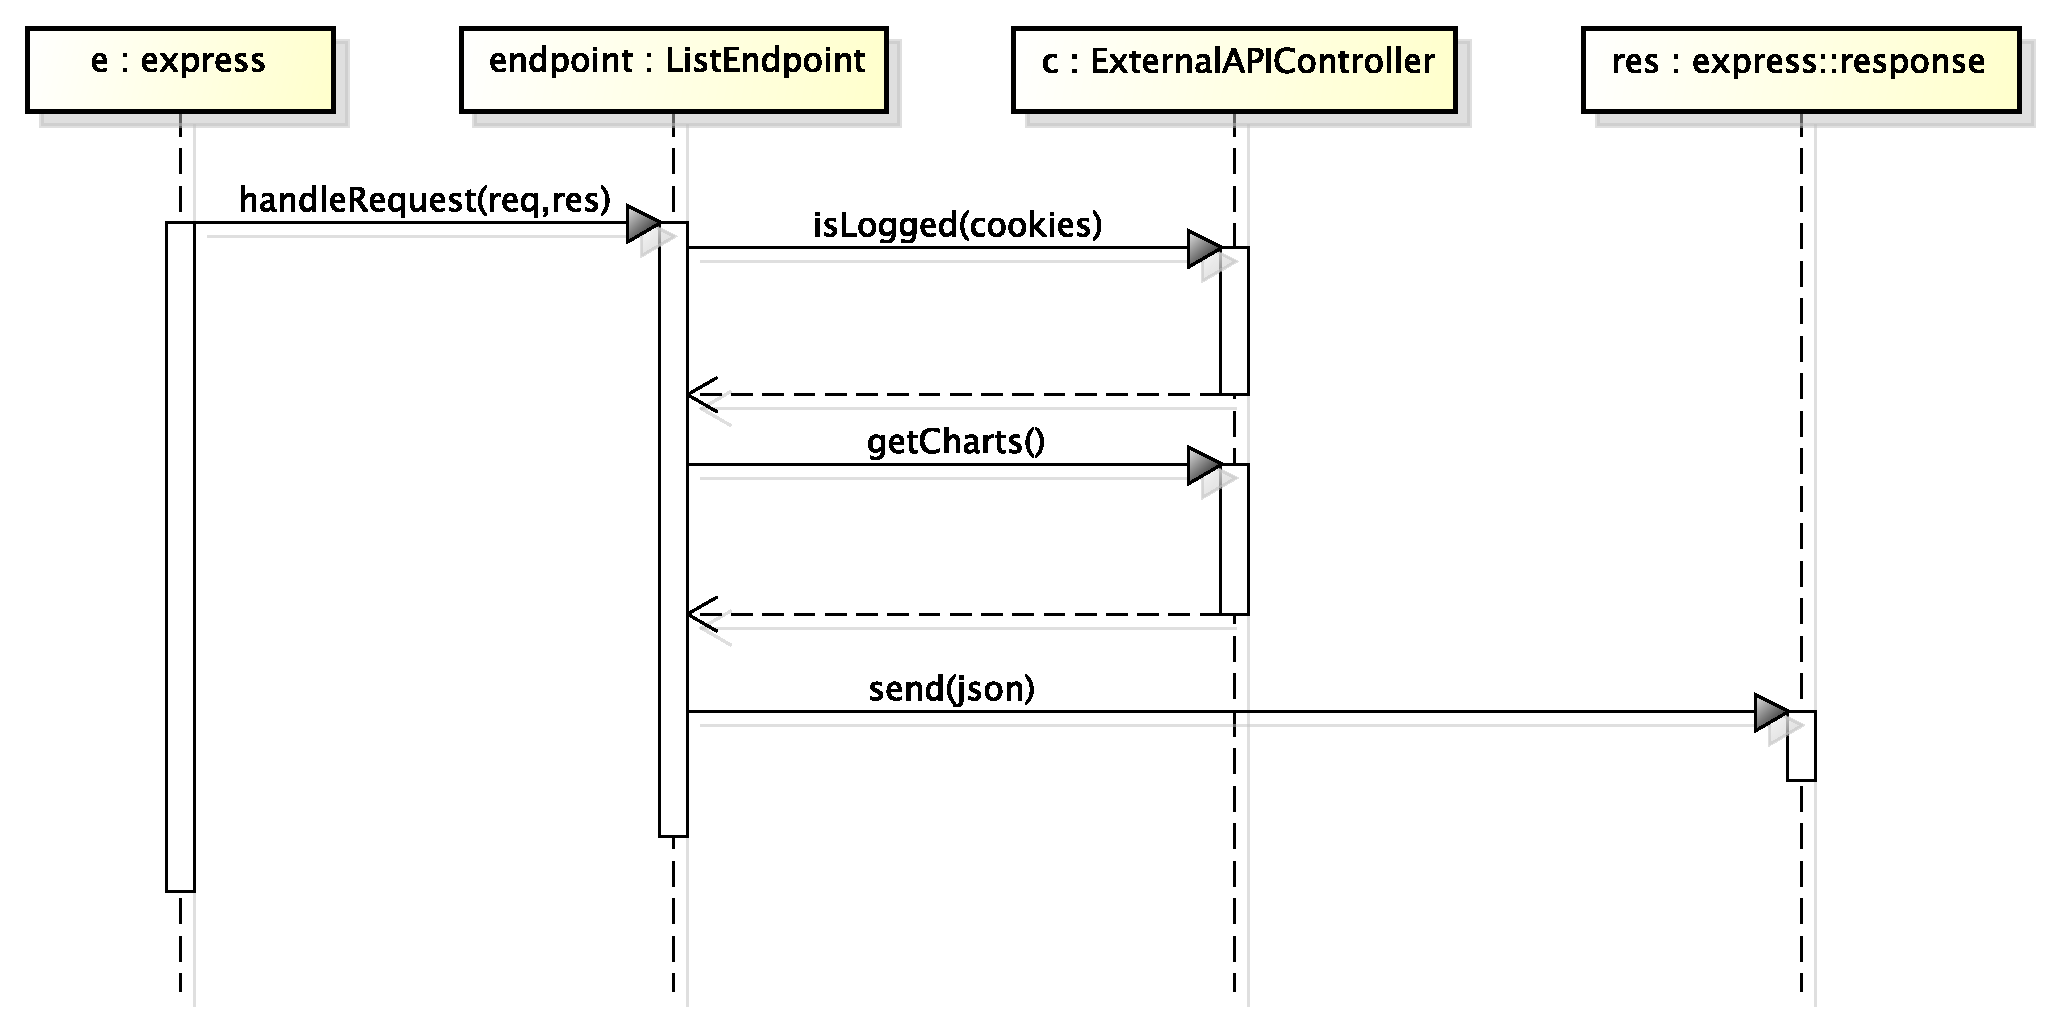
\includegraphics[scale=0.3]{DefinizioneDiProdotto/Pics/NorrisInvioLista}
                \caption{Diagramma di sequenza - Norris, invio lista}
            \end{figure}

            
        \level{3}{Invio di un chart}
        	Tale diagramma descrive come viene gestita la richiesta di un chart da parte di un \insglo{client} dal sistema \insglo{Norris}.
            \begin{figure}[H]
                \centering
                \includegraphics[scale=0.3]{DefinizioneDiProdotto/Pics/NorrisInvioChart}
                \caption{Diagramma di sequenza - Norris, invio chart}
            \end{figure}


    \level{3}{Classi aggiuntive}
        Per quanto riguarda le classi aggiuntive riguardanti che implementano i tipi “ChartSettings” e “ChartUpdate” si faccia riferimento all'appendice \nameref{app:schemi}, nella quale sono presenti gli schemi \insglo{JSON} di tali oggetti.
        
			\level{4}[NorrisSettingsImpl]{NorrisAggiuntive::NorrisSettingsImpl}
			

		\IfFileExists{DefinizioneDiProdotto/Pics/ClassiAggiuntive/NorrisSettingsImpl.pdf}{
			\begin{figure}[H]
				\centering
				\includegraphics[scale=0.5]{DefinizioneDiProdotto/Pics/ClassiAggiuntive/NorrisSettingsImpl}
				\caption{NorrisSettingsImpl}
			\end{figure}
		}
	
			
			\begin{itemize}
			\item \textbf{Nome:} NorrisSettingsImpl
			\item \textbf{Tipo:} classe
			
		\item \textbf{Astratta:}
		no
			\item \textbf{Visibilità:} public
			\item \textbf{Descrizione:} La classe NorrisSettingsImpl definisce le impostazioni relative ad un'istanza di Norris. Lo sviluppatore può definire le funzioni che verranno eseguite per l'autenticazione.
			\item \textbf{Attributi:}
				\begin{itemize}
				\setlength{\itemsep}{5pt}
				
					\item[\ding{111}] {+login : Function} \\ [1mm] L'attributo login rappresenta la funzione che verrà eseguita per avviare la sessione di un utente.
					\item[\ding{111}] {+logout : Function} \\ [1mm] L'attributo login rappresenta la funzione che verrà eseguita per terminare la sessione di un utente.
					\item[\ding{111}] {+keepAlive : Function} \\ [1mm] L'attributo login rappresenta la funzione che verrà eseguita per rinnovare la sessione di un utente.
					\item[\ding{111}] {+isLogged : Function} \\ [1mm] L'attributo login rappresenta la funzione che verrà eseguita per verificare lo stato dela sessione di un utente.
					\item[\ding{111}] {+endpoint : String} \\ [1mm] L'attributo endpoint definisce il path al quale sono disponibili le API esterne.
					\item[\ding{111}] {+secret : String} \\ [1mm] L'attributo secret definisce la chiave di cifrature per i cookie firmati.
					\item[\ding{111}] {+origins : String[]} \\ [1mm] L'attributo origin definisce gli host attendibili, verso i quali saranno disponibili le API esterne.
				\end{itemize}
		
			\end{itemize}
	
			\level{4}[PageSettingsImpl]{NorrisAggiuntive::PageSettingsImpl}
			

		\IfFileExists{DefinizioneDiProdotto/Pics/ClassiAggiuntive/PageSettingsImpl.pdf}{
			\begin{figure}[H]
				\centering
				\includegraphics[scale=0.5]{DefinizioneDiProdotto/Pics/ClassiAggiuntive/PageSettingsImpl}
				\caption{PageSettingsImpl}
			\end{figure}
		}
	
			
			\begin{itemize}
			\item \textbf{Nome:} PageSettingsImpl
			\item \textbf{Tipo:} classe
			
		\item \textbf{Astratta:}
		no
			\item \textbf{Visibilità:} public
			\item \textbf{Descrizione:} La classe PageSettingsImpl definisce le impostazioni di una pagina di Norris.
			\item \textbf{Attributi:}
				\begin{itemize}
				\setlength{\itemsep}{5pt}
				
					\item[\ding{111}] {+title : String} \\ [1mm] L'attributo title rappresenta il titolo di una pagina di Norris.
					\item[\ding{111}] {+maxChartsRow : int} \\ [1mm] L'attributo title rappresenta il numero massimo di righe visualizzabili all'interno della pagina.
					\item[\ding{111}] {+maxChartsCol : int} \\ [1mm] L'attributo title rappresenta il numero massimo di colonne visualizzabili all'interno della pagina.
				\end{itemize}
		
			\end{itemize}
	

    \level{2}{Diagrammi di sequenza}
    	In tale sezione vengono presentati i diagrammi di sequenza, che hanno lo scopo di descrivere scenari (determinate sequenze di azioni in cui tutte le scelte sono già state effettuate). Essi vengono usati per descrivere le relazioni che intercorrono, in termini di messaggi, tra attori, oggetti ed entità del sistema \insglo{Norris}.
        \level{3}{Creazione di un chart}
        	Tale diagramma descrive come viene creato un chart di un certo tipo prefissato.
            \begin{figure}[H]
                \centering
                \includegraphics[scale=0.3]{DefinizioneDiProdotto/Pics/NorrisCreazioneChart}
                \caption{Diagramma di sequenza - Norris, creazione chart}
            \end{figure}


        \level{3}{Aggiornamento di un chart}
        	Tale diagramma descrive come viene aggiornato un chart di un certo tipo (sulla base delle modalità di aggiornamento definite per quel tipo di grafico).
            \begin{figure}[H]
                \centering
                \includegraphics[scale=0.3]{DefinizioneDiProdotto/Pics/NorrisAggiornamentoChart}
                \caption{Diagramma di sequenza - Norris, aggiornamento chart}
            \end{figure}

            
        \level{3}{Invio lista dei grafici}
        	Tale diagramma descrive come viene gestita la richiesta della lista di tutti i grafici contenuti in una certa istanza di \insglo{Norris}.
            \begin{figure}[H]
                \centering
                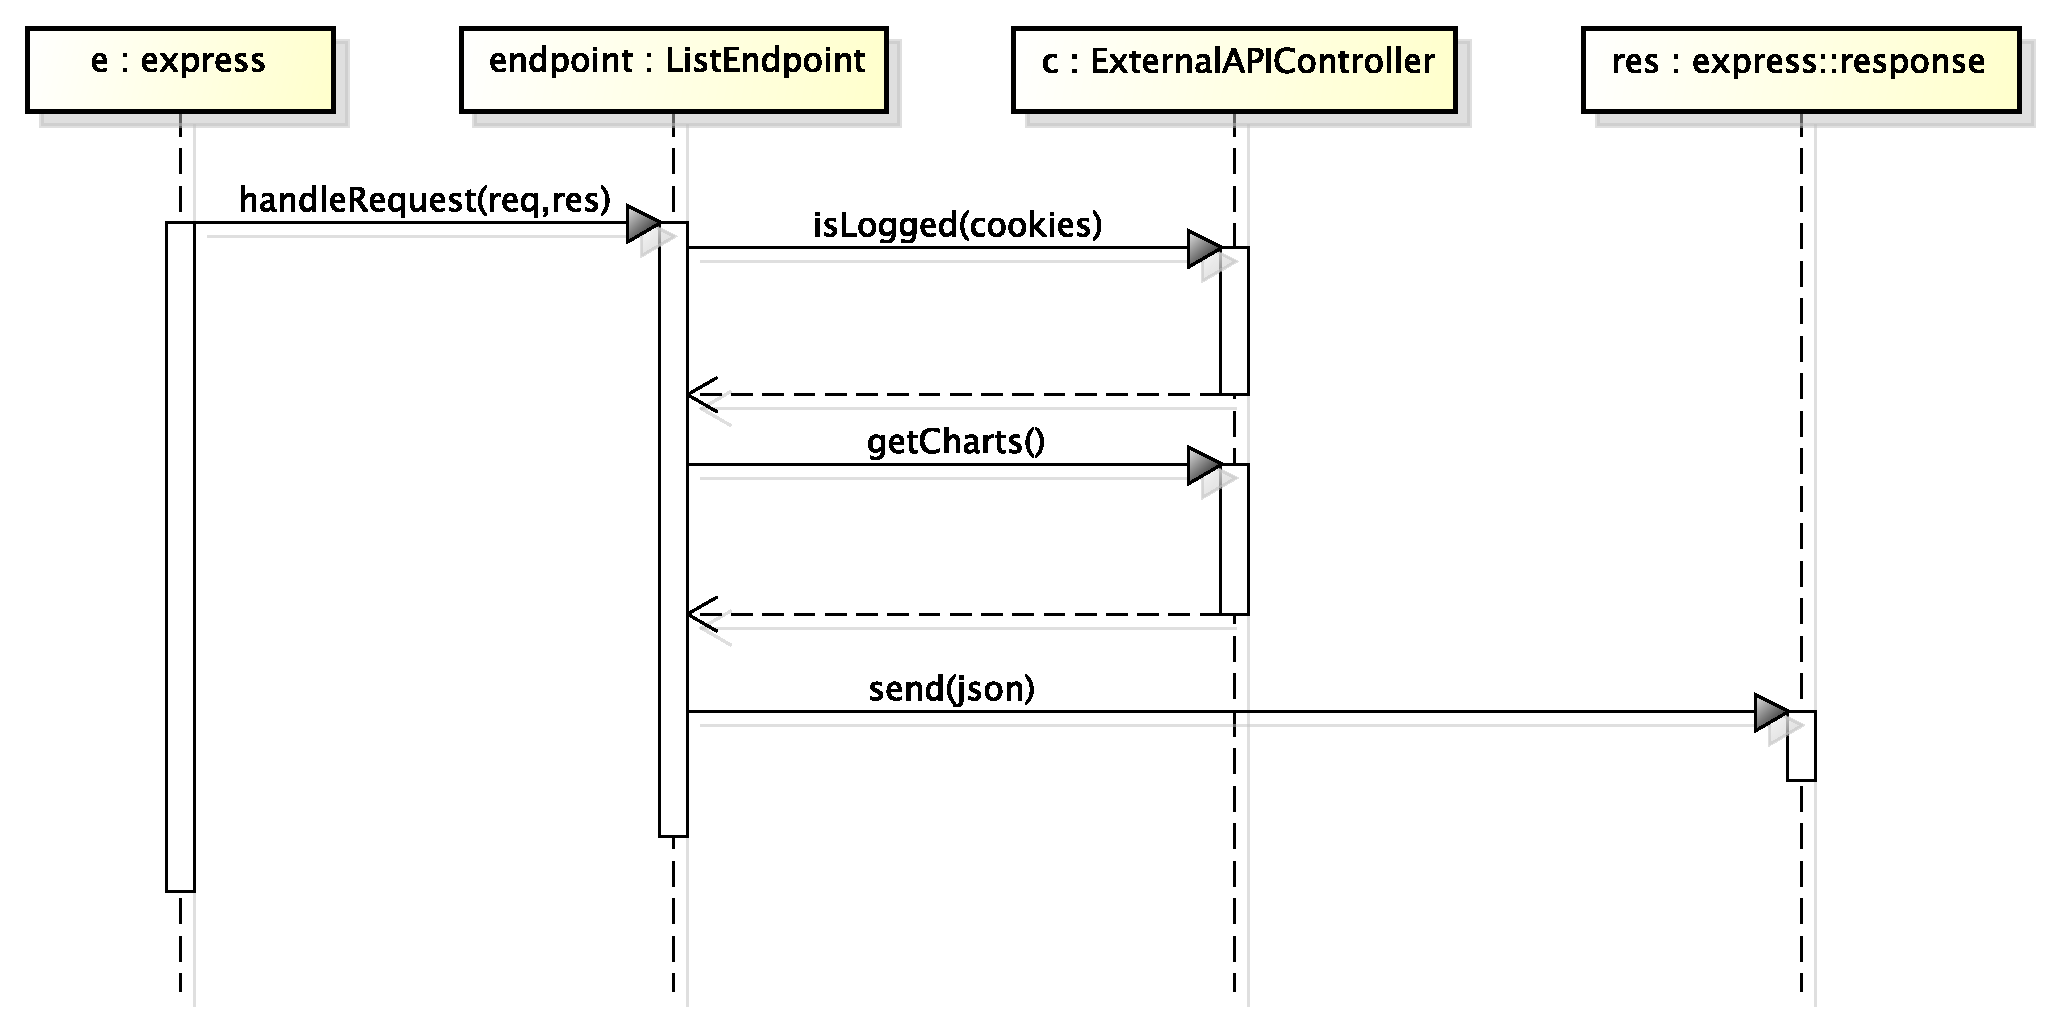
\includegraphics[scale=0.3]{DefinizioneDiProdotto/Pics/NorrisInvioLista}
                \caption{Diagramma di sequenza - Norris, invio lista}
            \end{figure}

            
        \level{3}{Invio di un chart}
        	Tale diagramma descrive come viene gestita la richiesta di un chart da parte di un \insglo{client} dal sistema \insglo{Norris}.
            \begin{figure}[H]
                \centering
                \includegraphics[scale=0.3]{DefinizioneDiProdotto/Pics/NorrisInvioChart}
                \caption{Diagramma di sequenza - Norris, invio chart}
            \end{figure}


    \level{3}{Classi aggiuntive}
        Per quanto riguarda le classi aggiuntive riguardanti che implementano i tipi “ChartSettings” e “ChartUpdate” si faccia riferimento all'appendice \nameref{app:schemi}, nella quale sono presenti gli schemi \insglo{JSON} di tali oggetti.
        
			\level{4}[NorrisSettingsImpl]{NorrisAggiuntive::NorrisSettingsImpl}
			

		\IfFileExists{DefinizioneDiProdotto/Pics/ClassiAggiuntive/NorrisSettingsImpl.pdf}{
			\begin{figure}[H]
				\centering
				\includegraphics[scale=0.5]{DefinizioneDiProdotto/Pics/ClassiAggiuntive/NorrisSettingsImpl}
				\caption{NorrisSettingsImpl}
			\end{figure}
		}
	
			
			\begin{itemize}
			\item \textbf{Nome:} NorrisSettingsImpl
			\item \textbf{Tipo:} classe
			
		\item \textbf{Astratta:}
		no
			\item \textbf{Visibilità:} public
			\item \textbf{Descrizione:} La classe NorrisSettingsImpl definisce le impostazioni relative ad un'istanza di Norris. Lo sviluppatore può definire le funzioni che verranno eseguite per l'autenticazione.
			\item \textbf{Attributi:}
				\begin{itemize}
				\setlength{\itemsep}{5pt}
				
					\item[\ding{111}] {+login : Function} \\ [1mm] L'attributo login rappresenta la funzione che verrà eseguita per avviare la sessione di un utente.
					\item[\ding{111}] {+logout : Function} \\ [1mm] L'attributo login rappresenta la funzione che verrà eseguita per terminare la sessione di un utente.
					\item[\ding{111}] {+keepAlive : Function} \\ [1mm] L'attributo login rappresenta la funzione che verrà eseguita per rinnovare la sessione di un utente.
					\item[\ding{111}] {+isLogged : Function} \\ [1mm] L'attributo login rappresenta la funzione che verrà eseguita per verificare lo stato dela sessione di un utente.
					\item[\ding{111}] {+endpoint : String} \\ [1mm] L'attributo endpoint definisce il path al quale sono disponibili le API esterne.
					\item[\ding{111}] {+secret : String} \\ [1mm] L'attributo secret definisce la chiave di cifrature per i cookie firmati.
					\item[\ding{111}] {+origins : String[]} \\ [1mm] L'attributo origin definisce gli host attendibili, verso i quali saranno disponibili le API esterne.
				\end{itemize}
		
			\end{itemize}
	
			\level{4}[PageSettingsImpl]{NorrisAggiuntive::PageSettingsImpl}
			

		\IfFileExists{DefinizioneDiProdotto/Pics/ClassiAggiuntive/PageSettingsImpl.pdf}{
			\begin{figure}[H]
				\centering
				\includegraphics[scale=0.5]{DefinizioneDiProdotto/Pics/ClassiAggiuntive/PageSettingsImpl}
				\caption{PageSettingsImpl}
			\end{figure}
		}
	
			
			\begin{itemize}
			\item \textbf{Nome:} PageSettingsImpl
			\item \textbf{Tipo:} classe
			
		\item \textbf{Astratta:}
		no
			\item \textbf{Visibilità:} public
			\item \textbf{Descrizione:} La classe PageSettingsImpl definisce le impostazioni di una pagina di Norris.
			\item \textbf{Attributi:}
				\begin{itemize}
				\setlength{\itemsep}{5pt}
				
					\item[\ding{111}] {+title : String} \\ [1mm] L'attributo title rappresenta il titolo di una pagina di Norris.
					\item[\ding{111}] {+maxChartsRow : int} \\ [1mm] L'attributo title rappresenta il numero massimo di righe visualizzabili all'interno della pagina.
					\item[\ding{111}] {+maxChartsCol : int} \\ [1mm] L'attributo title rappresenta il numero massimo di colonne visualizzabili all'interno della pagina.
				\end{itemize}
		
			\end{itemize}
	

    \level{2}{Diagrammi di sequenza}
    	In tale sezione vengono presentati i diagrammi di sequenza, che hanno lo scopo di descrivere scenari (determinate sequenze di azioni in cui tutte le scelte sono già state effettuate). Essi vengono usati per descrivere le relazioni che intercorrono, in termini di messaggi, tra attori, oggetti ed entità del sistema \insglo{Norris}.
        \level{3}{Creazione di un chart}
        	Tale diagramma descrive come viene creato un chart di un certo tipo prefissato.
            \begin{figure}[H]
                \centering
                \includegraphics[scale=0.3]{DefinizioneDiProdotto/Pics/NorrisCreazioneChart}
                \caption{Diagramma di sequenza - Norris, creazione chart}
            \end{figure}


        \level{3}{Aggiornamento di un chart}
        	Tale diagramma descrive come viene aggiornato un chart di un certo tipo (sulla base delle modalità di aggiornamento definite per quel tipo di grafico).
            \begin{figure}[H]
                \centering
                \includegraphics[scale=0.3]{DefinizioneDiProdotto/Pics/NorrisAggiornamentoChart}
                \caption{Diagramma di sequenza - Norris, aggiornamento chart}
            \end{figure}

            
        \level{3}{Invio lista dei grafici}
        	Tale diagramma descrive come viene gestita la richiesta della lista di tutti i grafici contenuti in una certa istanza di \insglo{Norris}.
            \begin{figure}[H]
                \centering
                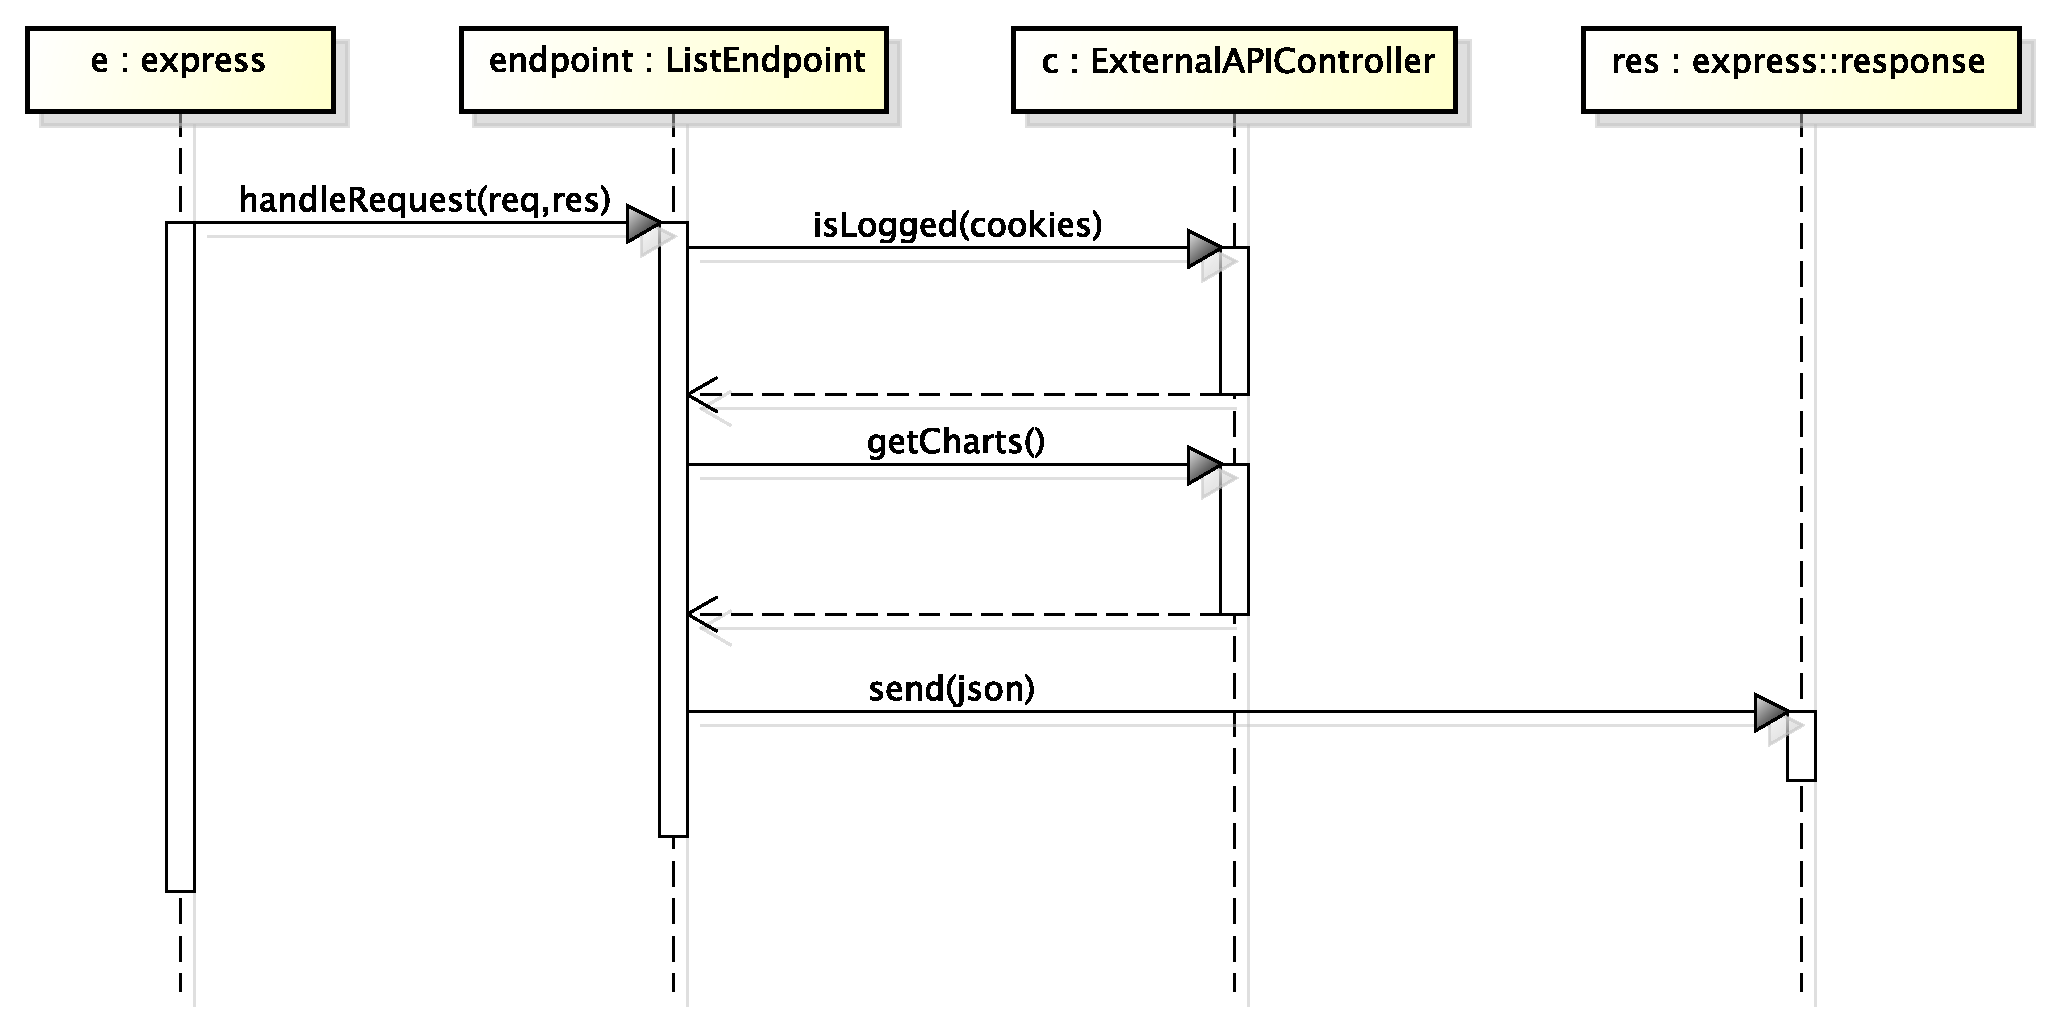
\includegraphics[scale=0.3]{DefinizioneDiProdotto/Pics/NorrisInvioLista}
                \caption{Diagramma di sequenza - Norris, invio lista}
            \end{figure}

            
        \level{3}{Invio di un chart}
        	Tale diagramma descrive come viene gestita la richiesta di un chart da parte di un \insglo{client} dal sistema \insglo{Norris}.
            \begin{figure}[H]
                \centering
                \includegraphics[scale=0.3]{DefinizioneDiProdotto/Pics/NorrisInvioChart}
                \caption{Diagramma di sequenza - Norris, invio chart}
            \end{figure}

		\level{4}{Classi aggiuntive Norris}
	Le interfacce \insglo{Norris}::DataModel::ChartData, \insglo{Norris}::DataModel::ChartSettings e \insglo{Norris}::DataModel::ChartUpdate rappresentano genericamente i vari oggetti che utilizzeremo per rappresentare i dati, le impostazioni e gli aggiornamamenti. Tali oggetti sono nel formato \insglo{JSON} ed essendo molto numerosi abbiamo deciso di non inserirle nel diagramma ma di elencarle e descriverle di seguito.

	\begin{itemize}
		\item \textbf{Norris::DataModel::NorrisChart::BarChartData} Questa classe implementa l'interfaccia \insglo{Norris}::DataModel::ChartData. Essa si occupa di rappresentare i dati di un grafico \insglo{bar chart};

		\item \textbf{\insglo{Norris}::DataModel::NorrisChart::LineChartData} Questa classe implementa l'interfaccia \insglo{Norris}::DataModel::ChartData. Essa si occupa di rappresentare i dati di un grafico \insglo{line chart};

		\item \textbf{\insglo{Norris}::DataModel::NorrisChart::MapChartData} Questa classe implementa l'interfaccia \insglo{Norris}::DataModel::ChartData. Essa si occupa di rappresentare i dati di un grafico \insglo{map chart};

		\item \textbf{\insglo{Norris}::DataModel::NorrisChart::TableData} Questa classe implementa l'interfaccia \linebreak \insglo{Norris}::DataModel::ChartData. Essa si occupa di rappresentare i dati di un grafico \insglo{table};

		\item \textbf{\insglo{Norris}::DataModel::NorrisChart::BarChartSetting} Questa classe implementa l'interfaccia \insglo{Norris}::DataModel::ChartSettings. Essa rappresenta le impostazioni di un grafico di tipo \insglo{bar chart};

		\item \textbf{\insglo{Norris}::DataModel::NorrisChart::LineChartSetting} Questa classe implementa l'interfaccia \insglo{Norris}::DataModel::ChartSettings. Essa rappresenta le impostazioni di un grafico di tipo \insglo{line chart};

		\item \textbf{\insglo{Norris}::DataModel::NorrisChart::MapChartSetting} Questa classe implementa l'interfaccia \insglo{Norris}::DataModel::ChartSettings. Essa rappresenta le impostazioni di un grafico di tipo \insglo{map chart};

		\item \textbf{\insglo{Norris}::DataModel::NorrisChart::TableSetting} Questa classe implementa l'interfaccia \insglo{Norris}::DataModel::ChartSettings. Essa rappresenta le impostazioni di un grafico di tipo \insglo{table};

		\item \textbf{\insglo{Norris}::DataModel::NorrisChart::BarChartInPlaceUpdate} Questa classe implementa l'interfaccia \insglo{Norris}::DataModel::ChartUpdate. Essa rappresenta un pacchetto di aggiornamento di tipo \insglo{in place} per un grafico di tipo \insglo{bar chart};

		\item \textbf{\insglo{Norris}::DataModel::NorrisChart::LineChartInPlaceUpdate} Questa classe implementa l'interfaccia \insglo{Norris}::DataModel::ChartUpdate. Essa rappresenta un pacchetto di aggiornamento di tipo \insglo{in place} per un grafico di tipo \insglo{line chart};

		\item \textbf{\insglo{Norris}::DataModel::NorrisChart::LineChartStreamUpdate} Questa classe implementa l'interfaccia \insglo{Norris}::DataModel::ChartUpdate. Essa rappresenta un pacchetto di aggiornamento di tipo \insglo{stream} per un grafico di tipo \insglo{line chart};

		\item \textbf{\insglo{Norris}::DataModel::NorrisChart::MapChartInPlaceUpdate} Questa classe implementa l'interfaccia \insglo{Norris}::DataModel::ChartUpdate. Essa rappresenta un pacchetto di aggiornamento di tipo \insglo{in place} per un grafico di tipo \insglo{map chart};

		\item \textbf{\insglo{Norris}::DataModel::NorrisChart::MapChartMovieUpdate} Questa classe implementa l'interfaccia \insglo{Norris}::DataModel::ChartUpdate. Essa rappresenta un pacchetto di aggiornamento di tipo \insglo{movie} per un grafico di tipo \insglo{map chart};

		\item \textbf{\insglo{Norris}::DataModel::NorrisChart::TableStreamUpdate} Questa classe implementa l'interfaccia \insglo{Norris}::DataModel::ChartUpdate. Essa rappresenta un pacchetto di aggiornamento di tipo \insglo{stream} per un grafico di tipo \insglo{table};

		\item \textbf{\insglo{Norris}::DataModel::NorrisChart::TableInPlaceUpdate} Questa classe implementa l'interfaccia \insglo{Norris}::DataModel::ChartUpdate. Essa rappresenta un pacchetto di aggiornamento di tipo \insglo{in place} per un grafico di tipo \insglo{table}.
	\end{itemize}

		\level{3}{Interazioni tra classi dei componenti di Norris}
	Il seguente diagramma UML rappresenta le interazioni tra le classi dei vari componenti di Norris.\\
	Alcune classi non sono state volontariamente inserite per rendere più comprendibile il diagramma.
	\begin{figure}[H]\centering
		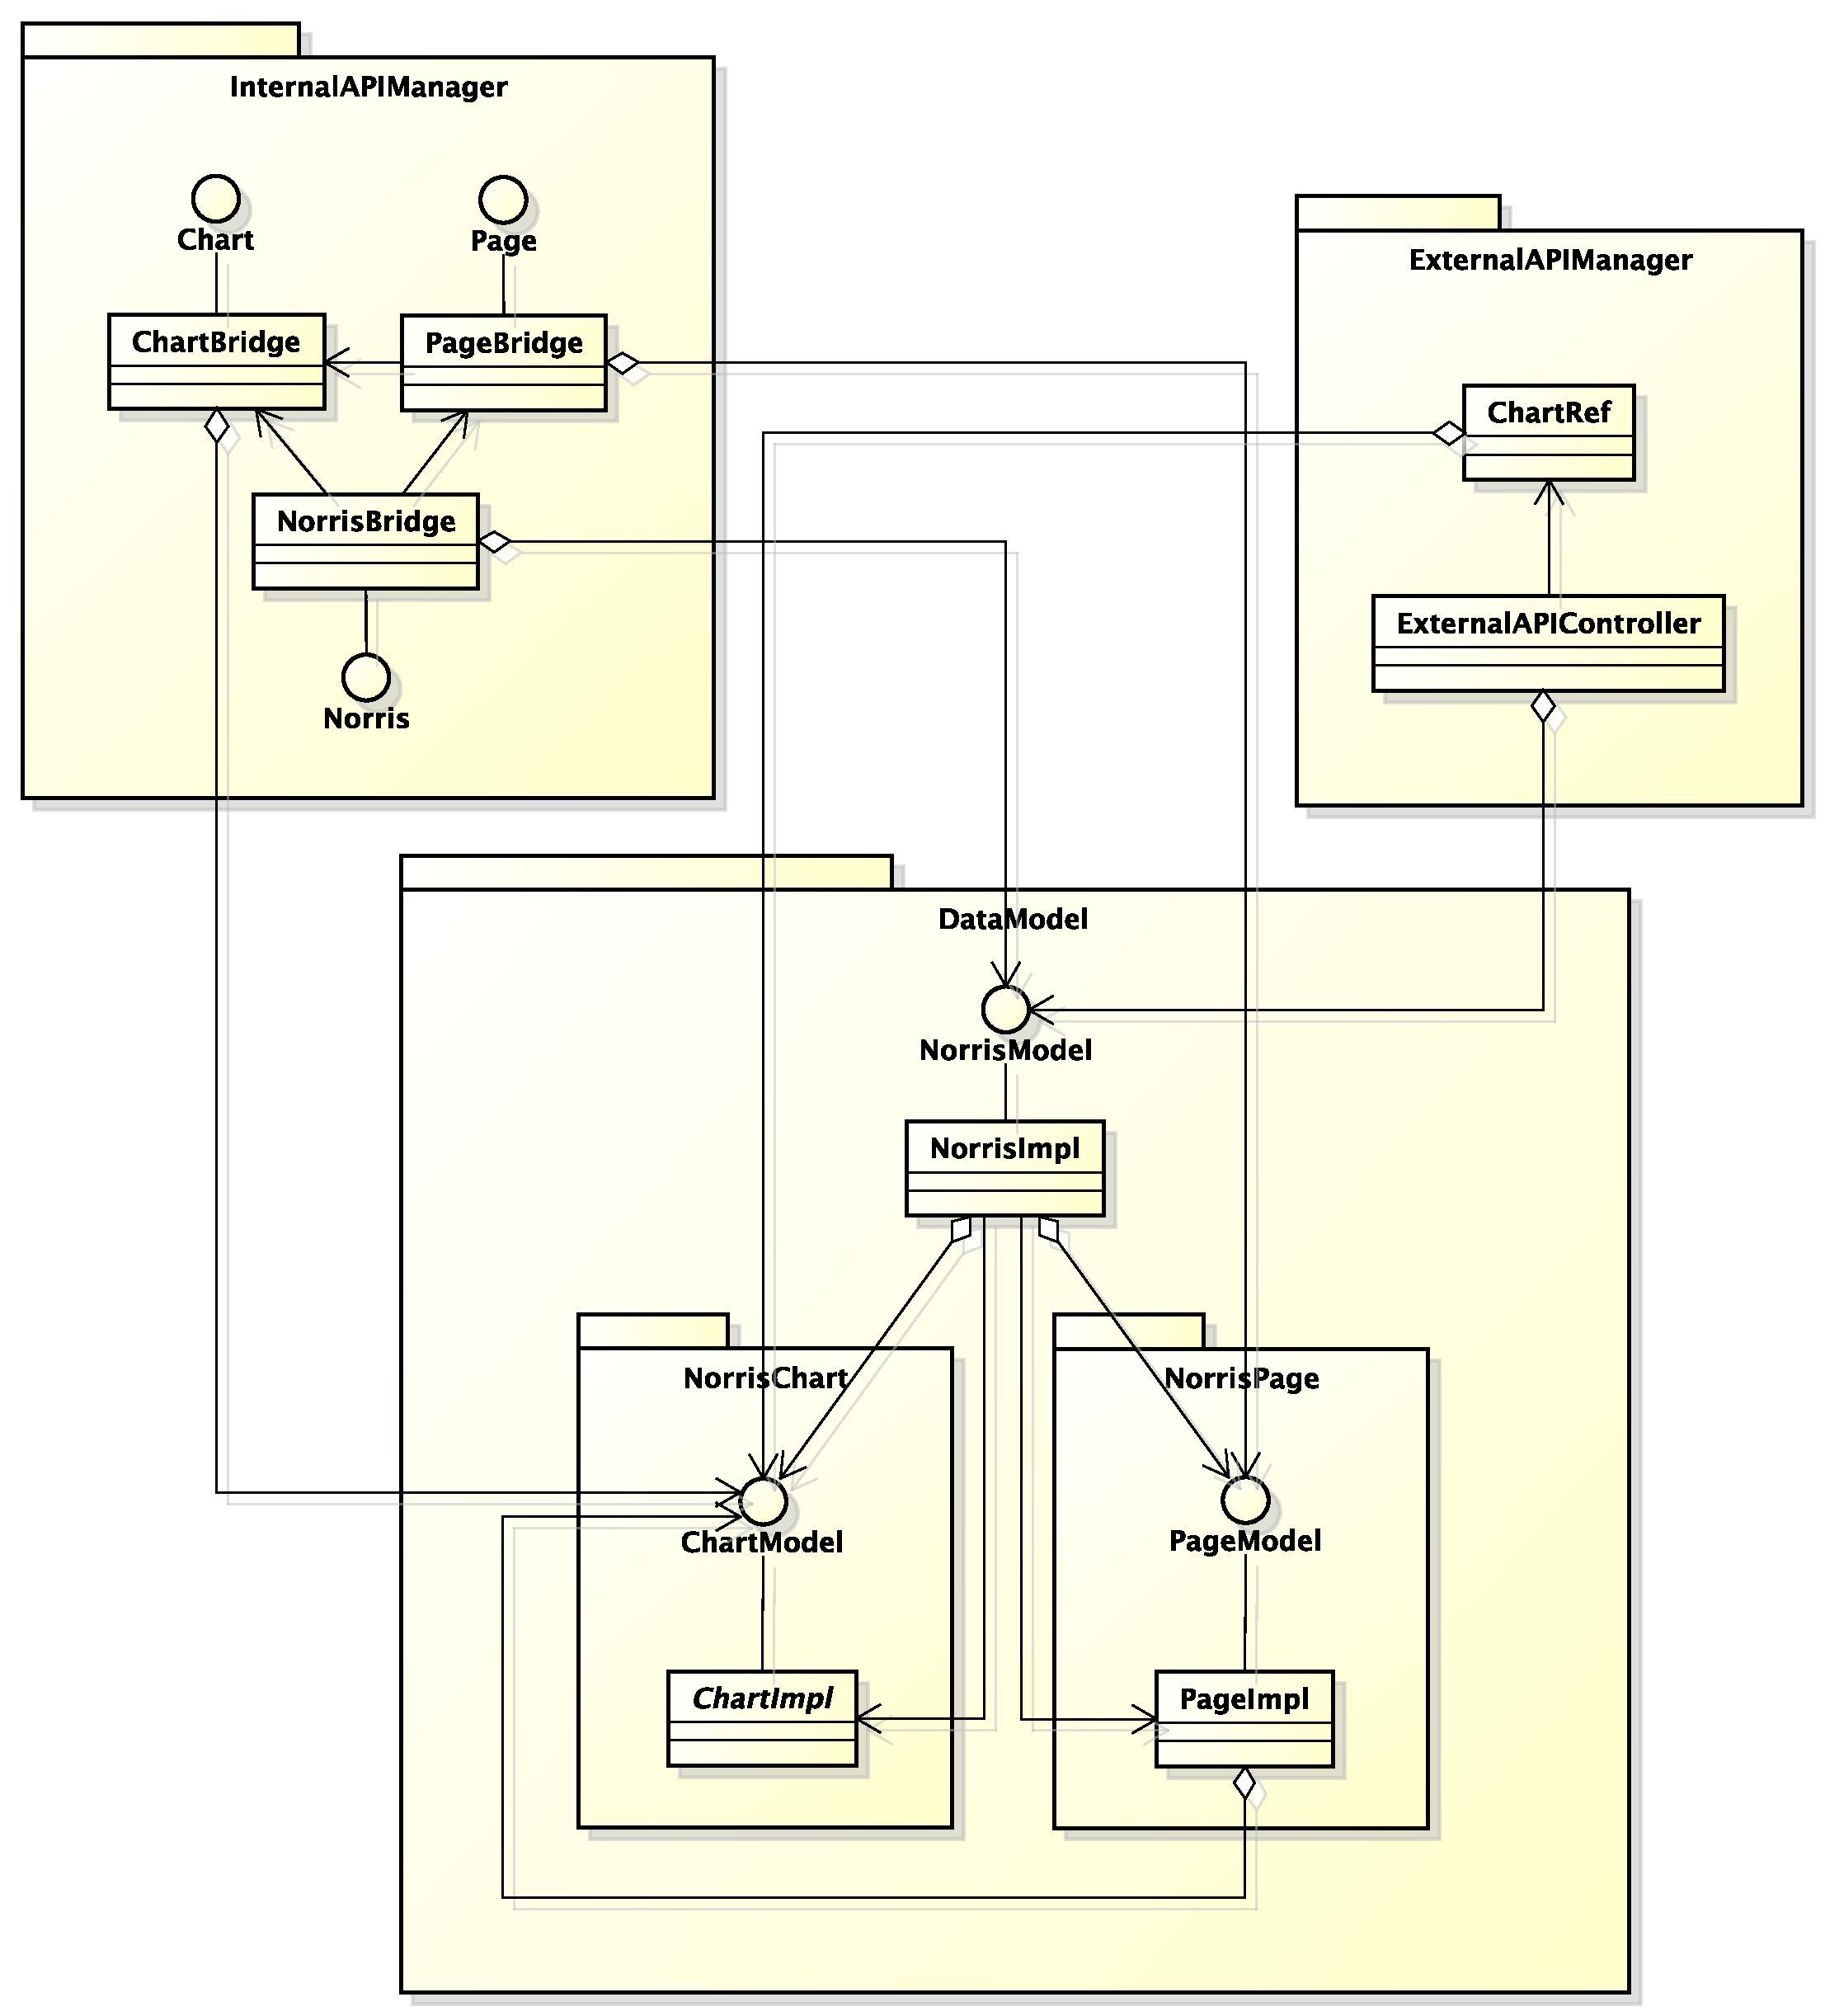
\includegraphics[width=\textwidth]{SpecificaTecnica/Pics/InterazioniComponentiNorris.pdf}
		\caption{Diagramma delle interazioni tra classi di componenti di Norris}
	\end{figure}

		
	\level{2}{Chuck}
		In questa sezione sono presenti le descrizioni di tutte le classi presenti all'interno del prodotto Chuck. Queste sono state suddivise in base al componente nelle quali sono contenute.
		
		\level{3}{Design pattern utilizzati}
Nella progettazione delle classi di Chuck abbiamo deciso di utilizzare alcuni design pattern. Riportiamo di seguito una loro breve descrizione e il contesto nel quale sono stati utilizzati.
\level{4}{Observer}
	L'Observer è un pattern comportamentale che ha lo scopo di monitorare lo stato di diversi oggetti legati ad un soggetto.
	Per la descrizione del pattern e dei vantaggi derivanti dalla sua applicazione si rimanda all'appendice \nameref{app:observer}.
	\level{5}{Contesto di utilizzo}
	Il pattern Observer si basa sugli oggetti “osservabili” e sugli “osservatori”. \\In Chuck il nucleo dell'implementazione dell'Observer si trova nel package Utils, in cui sono contenute le interfacce Observer e Observable, e la classe ObservableImpl che è l'implementazione di Observable. Questi tre elementi vengono poi estesi o implementati dagli altri elementi della libreria per realizzare il pattern completo.\\
	Interfacce che estendono Observable:
	\begin{itemize}
	\item ChartView::View;
	\item DataModel::ChartModel.
	\end{itemize}
	Interfacce che estendono Observer:
	\begin{itemize}
	\item ChartView::View.
	\end{itemize}
	Classi che estendono ObservableImpl:
	\begin{itemize}
	\item ChartView::ViewImpl;
	\item DataModel::ChartImpl.
	\end{itemize}
\level{4}{Bridge}
	Il Bridge è un pattern strutturale pensato per separare l'interfaccia di una classe dalla sua implementazione.\\ Per la descrizione del pattern e dei vantaggi derivanti dalla sua applicazione si rimanda all'appendice \nameref{app:bridge}.
	\level{5}{Contesto di utilizzo}
	In Chuck questo pattern viene utilizzato nel package ChuckAPIManager per separare l'implementazione dei chart (presente nel package DataModel) dall'interfaccia fornita allo sviluppatore client.
\level{4}{Dependency Injection}
	Dependency Injection è un pattern architetturale il cui scopo è separare il comportamento di una componente dalla risoluzione delle sue dipendenze.\\
	Per la descrizione del pattern e dei vantaggi derivanti dalla sua applicazione si rimanda all'appendice \nameref{app:dependencyinjection}.
	\level{5}{Contesto di utilizzo}
	La Dependency Injection viene utilizzata con le classi che implementano le interfaccie DataModel::ChartFactory e DataModel::Updater. Attraverso queste classi vengono "iniettate" nella classe DataModel::ChartImpl rispettivamente le corrispondenze tra i tipi di grafico e le rispettive classi factory e le corrispondenze tra i diversi tipi di aggiornamenti e le classi che li implementano.
\level{4}{Singleton}
	Il Singleton è un pattern creazionale il cui scopo è permettere la creazione di una sola istanza di una classe e fornire un punto di accesso globale ad essa.\\
	Per la descrizione del pattern e dei vantaggi derivanti dalla sua applicazione si rimanda all'appendice \nameref{app:singleton}.
	\level{5}{Contesto di utilizzo}
	Le classi che implementano il Singleton sono quelle che si occupano di creare i diversi tipi di grafici. cioè:
	\begin{itemize}
	\item DataModel::BarChartFactory;
	\item DataModel::LineChartFactory;
	\item DataModel::MapChartFactory;
	\item DataModel::TableFactory.
	\end{itemize}
\level{4}{Abstract Factory}
	Il pattern creazionale Abstract Factory si occupa di fornire un'interfaccia per la creazione di famiglie di prodotti, senza dover specificare classi concrete. \\
	Per la descrizione del pattern e dei vantaggi derivanti dalla sua applicazione si rimanda all'appendice \nameref{app:abstractfactory}.
	\level{5}{Contesto di utilizzo}
	Gli elementi che implementano Abstract Factory sono:
	\begin{itemize}
	\item Interfacce:
		\begin{itemize}
			\item DataModel::ChartFactory, con cui vengono generati i diversi tipi di grafici.
		\end{itemize}
	\item Classi:
		\begin{itemize}
			\item DataModel::BarChartFactory;
			\item DataModel::LineChartFactory;
			\item DataModel::MapChartFactory;
			\item DataModel::TableFactory.
		\end{itemize}
	\end{itemize}
\level{4}{Adapter}
	Il pattern strutturale Adapter viene utilizzato per adattare l'interfaccia di una classe in un'altra.\\
	Per la descrizione del pattern e dei vantaggi derivanti dalla sua applicazione si rimanda all'appendice \nameref{app:adapter}.
	\level{5}{Contesto di utilizzo}
	In Chuck l'Adapter viene utilizzato per calare le varie librerie esterne nel contesto di \projectname{}, e nello specifico sono rappresentate dalle diverse View, quindi:
	\begin{itemize}
	\item View::BarChartView e View::LineChartView sono adattatori per Chart.js;
	\item View::MapChartView è un adattatore per OpenStreetMaps;
	\item View::TableView è un adattatore per Dynatable.
	\end{itemize}
	
		\level{2}{Chuck}
	\begin{figure}[H]\centering
        \includegraphics[width=\textwidth]{SpecificaTecnica/Pics/componentiChuck}
        \caption{Diagramma delle componenti di Chuck}
    \end{figure}
	\level{3}{Design Pattern utilizzati}
	Nella progettazione delle componenti di Chuck abbiamo deciso di utilizzare il design pattern MVC.
	MOTIVAZIONE
    \level{3}{Descrizione dei componenti di Chuck}
    	\level{4}{Chuck API Manager}
    		La componente Chuck Api Manager si occupa di implementare le funzionalità offerte dalle API di Chuck allo sviluppatore client. Queste funzionalità sono:
    		\begin{itemize}
						\item inserimento di nuovi grafici in un sito web;
						\item scelta del tag HTML in cui inserire un grafico;
						\item modifica di alcune impostazioni dei grafici;
						\item login;
						\item logout.
			\end{itemize}
    		Questa componente si occupa inoltre di gestire la comunicazione con Norris.
    		
    	\level{4}{Chart View}
    	La componente Chart View ha il compito di visualizzare i grafici all'interno della pagina web. I grafici possono essere del tipo Bar Chart, Line Chart, Map Chart e Table. Quando un grafico viene aggiornato, questa componente si occupa di aggiornare anche la sua visualizzazione nella pagina web.

    	\level{4}{Controller}
    	La componente Controller ha lo scopo di ricevere gli input provenienti dalla Chart View ed effettuarne la gestione. L'input consiste in un sottoinsieme di dataset scelti dall'utente che sta visualizzando la pagina web. Il Controller deve far sì che vengano visualizzati solo questi dataset, in modo da permettere all'utente di applicare un filtro sulle serie.

    	\level{4}{Data Model}
    	La componente Data Model è un modello che astrae i grafici visualizzati nella pagina web. In essa sono contenuti i dati riguardanti i grafici, assieme alle relative impostazioni. In particolare sono presenti i modelli di tutte le tipologie di chart implementati da Norris. Il Data Model fornisce per ciascuna tipologia di grafico i metodi per inserire i dati e configurare alcune impostazioni. 
    
	\level{3}{Descrizione delle interazioni tra le componenti}
	
		\level{4}{Chuck API Manager - Data Model}
		Quando il Web Developer utilizza le API di Chuck oppure quando arriva un messaggio da Norris, Chuck API Manager apporta le opportune modifiche al Data Model, in modo che quest'ultimo rispecchi costantemente lo stato dei grafici da visualizzare.

		\level{4}{Chart View - Data Model}
		Quando la Chart View deve aggiornare la visualizzazione del grafico, essa effettua una query sul Data Model per ottenere le nuove informazioni relative al grafico da aggiornare.

		\level{4}{Data Model - Chart View}
		Quando avviene una modifica nel Data Model, una notifica avvisa la Chart View dell'avvenuto cambiamento. In particolare ciò accade quando è stato inserito un nuovo grafico o quando è arrivato l'aggiornamento di un grafico già presente.

		\level{4}{Chart View - Controller}
		Quando la Chart View riceve un input dall'utente, una notifica avvisa il Controller in modo che intraprenda l'azione per gestirla.

		\level{4}{Controller - Chart View}
		In caso di necessità il controller può selezionare la Chart View da visualizzare.
		\level{4}{Controller - Data Model}
		Quando intraprende un'azione, il controller può effettuare delle modifiche nel Data Model. In particolare ciò accade quando si deve inserire un nuovo grafico o quando arriva l'aggiornamento di un grafico già presente.

		\level{4}{Classi aggiuntive Chuck}
	Le interfacce \ignoreglo{Chuck::Model::NorrisChart::ChartData}, \ignoreglo{Chuck::Model::NorrisChart::ChartSettings} e \ignoreglo{Chuck::Model::NorrisChart::ChartUpdate} rappresentano genericamente i vari oggetti che utilizzeremo per rappresentare i dati, le impostazioni e gli aggiornamenti. Tali oggetti sono nel formato \insglo{JSON} ed essendo molto numerosi abbiamo deciso di non inserirle nel diagramma ma di elencarle e descriverle di seguito.

	\begin{itemize}
		\item \ignoreglo{\textbf{Chuck::Model::NorrisChart::BarChartData}} Questa classe implementa l'interfaccia \linebreak \insglo{Chuck}::Model::NorrisChart::ChartData. Essa si occupa di rappresentare i dati di un grafico \insglo{bar chart};

		\item \ignoreglo{\textbf{Chuck::Model::NorrisChart::LineChartData}} Questa classe implementa l'interfaccia \linebreak \insglo{Chuck}::Model::NorrisChart::ChartData. Essa si occupa di rappresentare i dati di un grafico \insglo{line chart};

		\item \ignoreglo{\textbf{Chuck::Model::NorrisChart::MapChartData}} Questa classe implementa l'interfaccia \linebreak \insglo{Chuck}::Model::NorrisChart::ChartData. Essa si occupa di rappresentare i dati di un grafico \insglo{map chart};

		\item \ignoreglo{\textbf{Chuck::Model::NorrisChart::TableData}} Questa classe implementa l'interfaccia \linebreak \insglo{Chuck}::Model::NorrisChart::ChartData. Essa si occupa di rappresentare i dati di un grafico \insglo{table};

		\item \ignoreglo{\textbf{Chuck::Model::NorrisChart::BarChartSetting}} Questa classe implementa l'interfaccia \linebreak \insglo{Chuck}::Model::NorrisChart::ChartSettings. Essa rappresenta le impostazioni di un grafico di tipo \insglo{bar chart};

		\item \ignoreglo{\textbf{Chuck::Model::NorrisChart::LineChartSetting}} Questa classe implementa l'interfaccia \linebreak \insglo{Chuck}::Model::NorrisChart::ChartSettings. Essa rappresenta le impostazioni di un grafico di tipo \insglo{line chart};

		\item \ignoreglo{\textbf{Chuck::Model::NorrisChart::MapChartSetting}} Questa classe implementa l'interfaccia \linebreak \insglo{Chuck}::Model::NorrisChart::ChartSettings. Essa rappresenta le impostazioni di un grafico di tipo \insglo{map chart};

		\item \ignoreglo{\textbf{Chuck::Model::NorrisChart::TableSetting}} Questa classe implementa l'interfaccia \linebreak \insglo{Chuck}::Model::NorrisChart::ChartSettings. Essa rappresenta le impostazioni di un grafico di tipo \insglo{table};

		\item \ignoreglo{\textbf{Chuck::Model::NorrisChart::BarChartInPlaceUpdate}} Questa classe implementa l'interfaccia \insglo{Chuck}::Model::NorrisChart::ChartUpdate. Essa rappresenta un pacchetto di aggiornamento di tipo \insglo{in place} per un grafico di tipo \insglo{bar chart};

		\item \ignoreglo{\textbf{Chuck::Model::NorrisChart::LineChartInPlaceUpdate}} Questa classe implementa l'interfaccia \insglo{Chuck}::Model::NorrisChart::ChartUpdate. Essa rappresenta un pacchetto di aggiornamento di tipo \insglo{in place} per un grafico di tipo \insglo{line chart};

		\item \ignoreglo{\textbf{Chuck::Model::NorrisChart::LineChartStreamUpdate}} Questa classe implementa l'interfaccia \insglo{Chuck}::Model::NorrisChart::ChartUpdate. Essa rappresenta un pacchetto di aggiornamento di tipo \insglo{stream} per un grafico di tipo \insglo{line chart};

		\item \ignoreglo{\textbf{Chuck::Model::NorrisChart::MapChartInPlaceUpdate}} Questa classe implementa l'interfaccia \insglo{Chuck}::Model::NorrisChart::ChartUpdate. Essa rappresenta un pacchetto di aggiornamento di tipo \insglo{in place} per un grafico di tipo \insglo{map chart};

		\item \ignoreglo{\textbf{Chuck::Model::NorrisChart::MapChartMovieUpdate}} Questa classe implementa l'interfaccia \insglo{Chuck}::Model::NorrisChart::ChartUpdate. Essa rappresenta un pacchetto di aggiornamento di tipo \insglo{movie} per un grafico di tipo \insglo{map chart};

		\item \ignoreglo{\textbf{Chuck::Model::NorrisChart::TableStreamUpdate}} Questa classe implementa l'interfaccia \insglo{Chuck}::Model::NorrisChart::ChartUpdate. Essa rappresenta un pacchetto di aggiornamento di tipo \insglo{stream} per un grafico di tipo \insglo{table};

		\item \ignoreglo{\textbf{Chuck::Model::NorrisChart::TableInPlaceUpdate}} Questa classe implementa l'interfaccia \insglo{Chuck}::Model::NorrisChart::ChartUpdate. Essa rappresenta un pacchetto di aggiornamento di tipo \insglo{in place} per un grafico di tipo \insglo{table}.
	\end{itemize}

		\level{3}{Interazioni tra classi dei componenti di Chuck}
Il seguente diagramma UML rappresenta le interazioni tra le classi dei vari componenti di Chuck.\\
	Alcune classi non sono state volontariamente inserite per rendere più comprendibile il diagramma.

	\begin{figure}[H]\centering
		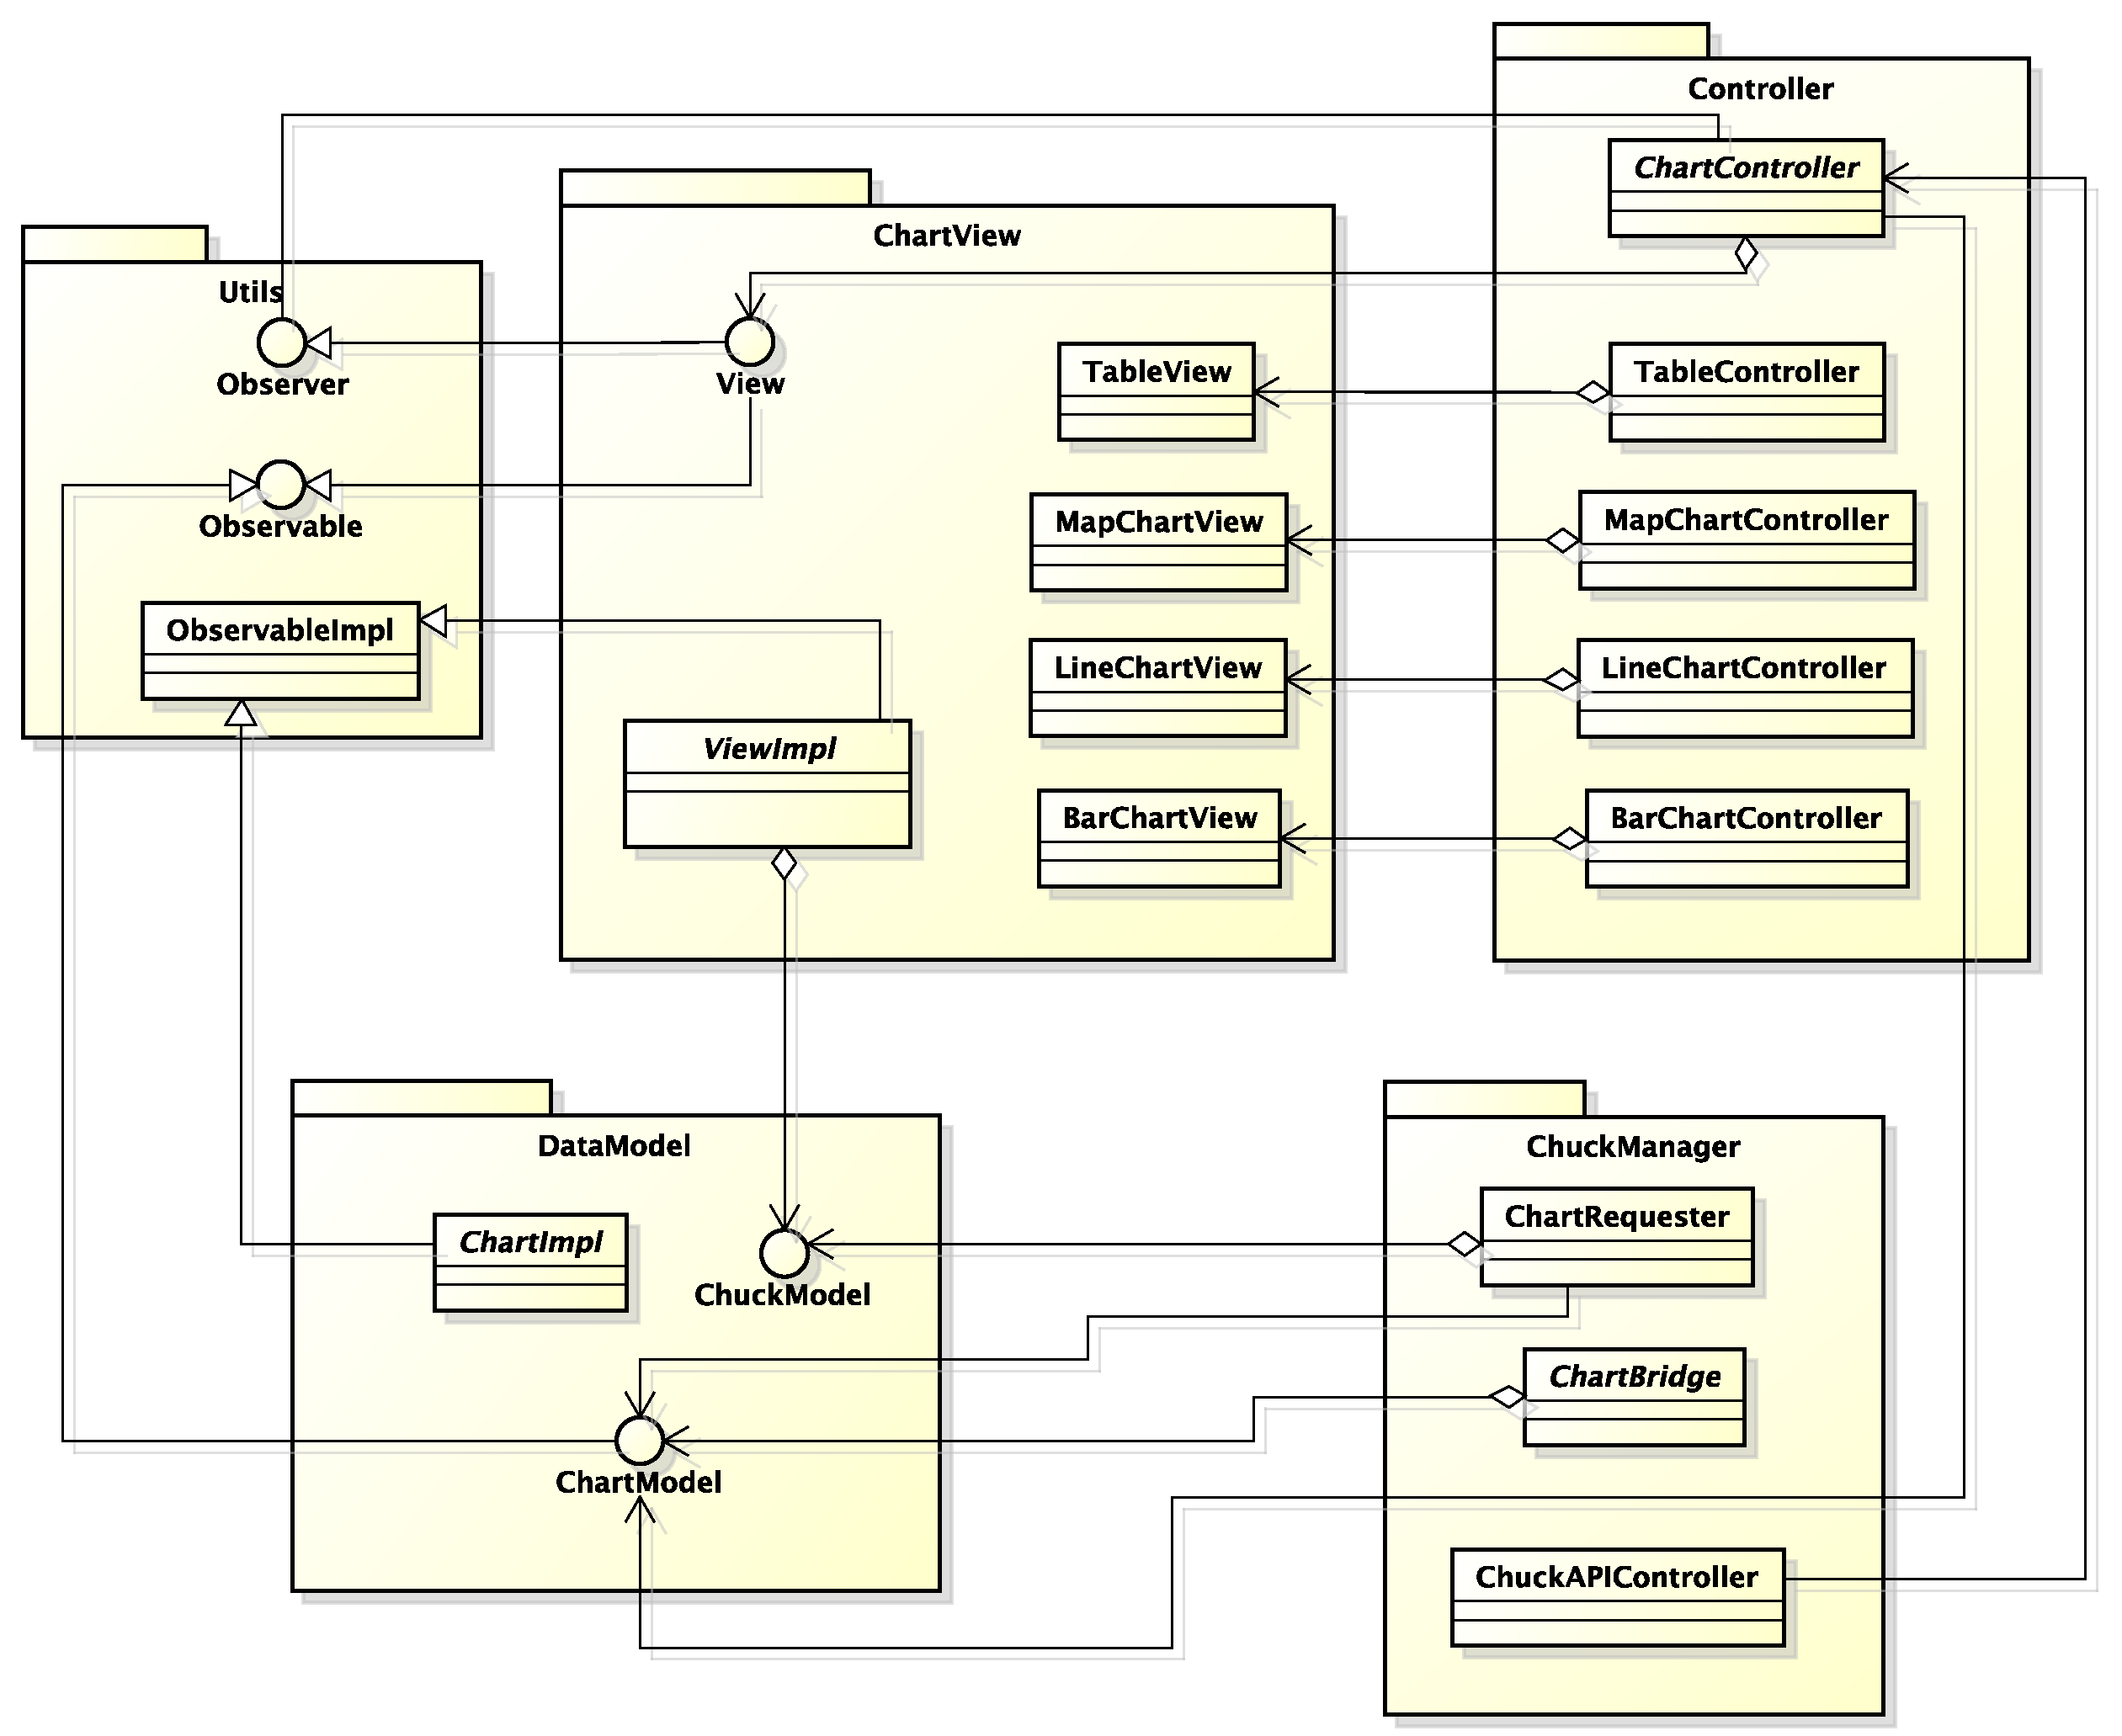
\includegraphics[width=\textwidth]{SpecificaTecnica/Pics/InterazioniComponentiChuck.pdf}
		\caption{Diagramma delle interazioni tra classi di componenti di Chuck}
	\end{figure}
	
	\level{2}{Applicazione Android}
		In questa sezione sono presenti le descrizioni di tutte le classi presenti all'interno dell'applicazione Android. Queste sono state suddivise in base al componente nelle quali sono contenute.
		\level{3}{Design pattern utilizzati}
Nella progettazione delle classi dell'applicazione abbiamo deciso di utilizzare alcuni design pattern. Riportiamo di seguito una loro breve descrizione e il contesto nel quale sono stati utilizzati.
\level{4}{Observer}
	L'Observer è un pattern comportamentale che ha lo scopo di monitorare lo stato di diversi oggetti legati ad un soggetto.
	Per la descrizione del pattern e dei vantaggi derivanti dalla sua applicazione si rimanda all'appendice \nameref{app:observer}.
	\level{5}{Contesto di utilizzo}
	Il pattern Observer si basa sugli oggetti “osservabili” e sugli “osservatori”. \\ Nell'applicazione Android il nucleo dell'implementazione dell'Observer si trova nel package Utils, in cui sono contenute le interfacce Utils::Observer e Utils::Observable, e la classe Utils::ObservableImpl (implementazione di Utils::Observable). Questi tre elementi vengono poi estesi o implementati dagli altri elementi della libreria per realizzare il pattern completo.\\
	Interfacce che estendono Observable:
	\begin{itemize}
	\item Model::Chart.
	\end{itemize}
	Classi che implementano Observer:
	\begin{itemize}
	\item Controller::Controller;
	\item View::ChartActivity.
	\end{itemize}
	Classi che estendono ObservableImpl:
	\begin{itemize}
	\item View::ObservableImpl;
	\item Model::ChartImpl.
	\end{itemize}
\level{4}{Dependency Injection}
	Dependency Injection è un pattern architetturale il cui scopo è separare il comportamento di una componente dalla risoluzione delle sue dipendenze.\\
	Per la descrizione del pattern e dei vantaggi derivanti dalla sua applicazione si rimanda all'appendice \nameref{app:dependencyinjection}.
	\level{5}{Contesto di utilizzo}
	La Dependency Injection viene utilizzata con le classi che implementano le seguenti interfacce:
	\begin{itemize}
	\item Controller::ControllerFactory, inietta in Controller::ChartController le corrispondenze tra i tipi di controller e le rispettive classi factory;
	\item Model::ChartFactory, inietta in Model::ChartImpl le  corrispondenze tra i tipi di grafico e le rispettive classi factory;
	\item Model::Updater, inietta in Model::ChartImpl le corrispondenze tra i diversi tipi di aggiornamenti e le classi che li implementano.
	\end{itemize}
\level{4}{Singleton}
	Il Singleton è un pattern creazionale il cui scopo è permettere la creazione di una sola istanza di una classe, nonchè di fornire un punto di accesso globale ad essa.\\
	Per la descrizione del pattern e dei vantaggi derivanti dalla sua applicazione si rimanda all'appendice \nameref{app:singleton}.
	\level{5}{Contesto di utilizzo}
	Nell'applicazione Android il Singleton viene implementato nella classe Controller::JSONParser.
\level{4}{Abstract Factory}
	Il pattern creazionale Abstract Factory si occupa di fornire un'interfaccia per la creazione di famiglie di prodotti, senza dover specificare classi concrete. \\
	Per la descrizione del pattern e dei vantaggi derivanti dalla sua applicazione si rimanda all'appendice \nameref{app:abstractfactory}.
	\level{5}{Contesto di utilizzo}
	Gli elementi che implementano Abstract Factory sono:
	\begin{itemize}
	\item Interfacce:
		\begin{itemize}
			\item Model::ChartFactory, con cui vengono generati i diversi tipi di grafici;
			\item Controller::ControllerFactory, con cui sono generati i diversi tipi di controller dei grafici.
		\end{itemize}
	\item Classi:
		\begin{itemize}
			\item Model::BarChartFactory;
			\item Model::LineChartFactory;
			\item Model::MapChartFactory;
			\item Model::TableFactory;
			\item Controller::BarChartControllerFactory;
			\item Controller::LineChartControllerFactory;
			\item Controller::MapChartControllerFactory;
			\item Controller::TableControllerFactory.
		\end{itemize}
	\end{itemize}
\level{4}{Adapter}
	Il pattern strutturale Adapter viene utilizzato per adattare l'interfaccia di una classe in un'altra.\\
	Per la descrizione del pattern e dei vantaggi derivanti dalla sua applicazione si rimanda all'appendice \nameref{app:adapter}.
	\level{5}{Contesto di utilizzo}
	Nell'applicazione Android l'Adapter viene utilizzato per calare le varie librerie esterne nel contesto di \projectname{}, e nello specifico sono rappresentate dalle diverse View, quindi:
	\begin{itemize}
	\item View::BarChartActivity è un adattatore per MPABarChart;
	\item View::MapChartActivity è un adattatore per GoogleMap Android API v2;
	\item View::LineChartActivity è un adattatore per MPALineChart.
	\end{itemize}
	
		\level{1}{Applicazione}

	\level{2}{Classi}
		\level{1}{Applicazione}

	\level{2}{Classi}
		\level{1}{Applicazione}

	\level{2}{Classi}
		\input{Classi/Applicazione.tex}
		\level{3}{Classi aggiuntive Applicazione}
	Le interfacce Applicazione::DataModel::DataObject, Applicazione::DataModel::SettingsObject e Applicazione::DataModel::UpdateObject rappresentano genericamente i vari oggetti che utilizzeremo per rappresentare i dati, le impostazioni e gli aggiornamamenti. Tali oggetti sono nel formato JSON ed essendo molto numerosi abbiamo deciso di non inserirle nel diagramma ma di elencarle e descriverle di seguito.

	\begin{itemize}
		\item \textbf{Applicazione::DataModel::BarChartDataObject} Questa classe implementa l'interfaccia Applicazione::DataModel::DataObject. Essa si occupa di rappresentare i dati di un grafico bar chart;

		\item \textbf{Applicazione::DataModel::LineChartDataObject} Questa classe implementa l'interfaccia Applicazione::DataModel::DataObject. Essa si occupa di rappresentare i dati di un grafico line chart;

		\item \textbf{Applicazione::DataModel::MapChartDataObject} Questa classe implementa l'interfaccia Applicazione::DataModel::DataObject. Essa si occupa di rappresentare i dati di un grafico map chart;

		\item \textbf{Applicazione::DataModel::TableDataObject} Questa classe implementa l'interfaccia Applicazione::DataModel::DataObject. Essa si occupa di rappresentare i dati di un grafico table;

		\item \textbf{Applicazione::DataModel::BarChartSettingObject} Questa classe implementa l'interfaccia Applicazione::DataModel::SettingObject. Essa rappresenta le impostazioni di un grafico di tipo bar chart;

		\item \textbf{Applicazione::DataModel::LineChartSettingObject} Questa classe implementa l'interfaccia Applicazione::DataModel::SettingObject. Essa rappresenta le impostazioni di un grafico di tipo line chart;

		\item \textbf{Applicazione::DataModel::MapChartSettingObject} Questa classe implementa l'interfaccia Applicazione::DataModel::SettingObject. Essa rappresenta le impostazioni di un grafico di tipo map chart;

		\item \textbf{Applicazione::DataModel::TableSettingObject} Questa classe implementa l'interfaccia Applicazione::DataModel::SettingObject. Essa rappresenta le impostazioni di un grafico di tipo table;

		\item \textbf{Applicazione::DataModel::BarChartInPlaceUpdateObject} Questa classe implementa l'interfaccia Applicazione::DataModel::UpdateObject. Essa rappresenta un pacchetto di aggiornamento di tipo in place per un grafico di tipo bar chart;

		\item \textbf{Applicazione::DataModel::LineChartInPlaceUpdateObject} Questa classe implementa l'interfaccia Applicazione::DataModel::UpdateObject. Essa rappresenta un pacchetto di aggiornamento di tipo in place per un grafico di tipo line chart;

		\item \textbf{Applicazione::DataModel::LineChartStreamUpdateObject} Questa classe implementa l'interfaccia Applicazione::DataModel::UpdateObject. Essa rappresenta un pacchetto di aggiornamento di tipo stream per un grafico di tipo line chart;

		\item \textbf{Applicazione::DataModel::MapChartInPlaceUpdateObject} Questa classe implementa l'interfaccia Applicazione::DataModel::UpdateObject. Essa rappresenta un pacchetto di aggiornamento di tipo in place per un grafico di tipo map chart;

		\item \textbf{Applicazione::DataModel::MapChartMovieUpdateObject} Questa classe implementa l'interfaccia Applicazione::DataModel::UpdateObject. Essa rappresenta un pacchetto di aggiornamento di tipo movie per un grafico di tipo map chart;

		\item \textbf{Applicazione::DataModel::TableStreamUpdateObject} Questa classe implementa l'interfaccia Applicazione::DataModel::UpdateObject. Essa rappresenta un pacchetto di aggiornamento di tipo stream per un grafico di tipo table;

		\item \textbf{Applicazione::DataModel::TableInPlaceUpdateObject} Questa classe implementa l'interfaccia Applicazione::DataModel::UpdateObject. Essa rappresenta un pacchetto di aggiornamento di tipo in place per un grafico di tipo table.
	\end{itemize}
		\level{3}{Interazioni tra classi dei componenti dell'applicazione Android}
	Dopo che sono stati descritte nel dettaglio tutte le varie classi necessarie alla progettazione dell'applicazione \insglo{Android}, è necessario mostrare come le classi appartenenti a componenti differenti interagiscano tra di loro. È quindi inserito in seguito un diagramma \insglo{UML} che rappresenta tutte le interazioni presenti tra i vari componenti.\\
	Si noti che alcune classi non sono state inserite in quanto si è voluto rendere più comprensibile il diagramma.

	\begin{figure}[H]\centering
		\includegraphics[width=\textwidth]{SpecificaTecnica/Pics/InterazioniComponentiApplicazione.pdf}
		\caption{Diagramma delle interazioni tra classi di componenti dell'Applicazione}
	\end{figure}
